%!TEX TS-program = xelatex
\documentclass[main]{subfiles}
%这是一个子文件,单独编译时会自动导入main文件的导言区
%这里可以放自定义命令,不会和别人的冲突请放心
%但是不能放newtheorem等高级命令,需要请在群里说
%下面是一些数学命令的简化,可以保留,可以删去,也可以按你的习惯修改
\usetikzlibrary{arrows.meta}
\usetikzlibrary{positioning}
\def\e{\textup{e}}
\def\i{\textup{i}}
\def\dif{\textup{d}}
\def\T{\textup{T}}
\def\diag{\textup{diag}}
\def\id{\textup{id}}
\newcommand{\toi}[1]{{#1}\to\infty}
\newcommand{\dis}{\displaystyle}
\newcommand{\bv}{\mathrm{BV}}
\newcommand{\ac}{\mathrm{AC}}
\newcommand{\mr}{\mathbb{R}}
\newcommand{\mn}{\mathbb{N}}
\newcommand{\mq}{\mathbb{Q}}
\newcommand{\mz}{\mathbb{Z}}
\newcommand{\rel}{\text{ rel }}
\newcommand{\sgn}{\operatorname{sign}}
\newcommand{\ve}{\varepsilon}
\newcommand{\bs}{\backslash}
\newcommand{\Span}{\operatorname{span}}
\renewcommand{\ll}{\lim\limits}
\renewcommand{\ker}{\operatorname{Ker}}
\renewcommand{\hom}{\operatorname{Hom}}
\renewcommand{\leq}{\leqslant}
\renewcommand{\geq}{\geqslant}
\begin{document}
\renewcommand{\filename}{素数定理}%在这里填你的文件名,避免\label冲突
%这里开始写你的代码
\section{素数定理}
\subsection*{背景介绍}
素数, 指在大于1的自然数中, 除了1和该数自身外, 无法被其他自然数整除的数。素数在数论中非常重要: 算术基本定理指出, 每个大于1的整数均可唯一的写成素数乘积, 即素数可被认为是自然数的“基本建材”.
在实际应用中, 素数不仅在公开密钥的算法中具有奠基性的作用, 而且在汽车, 导弹等等现代设备的设计中起着重要作用.
\par 关于素数有许多悬而未决的大问题, 比如大家耳熟能详的黎曼猜想, 哥德巴赫猜想, 孪生素数猜想$\cdots \cdots$ 素数分布是数论中研究素数性质的困难且重要的课题, 而素数定理描述了素数在自然数中分布的渐进情况. 简单来说就是前 $n$ 个数中有几个素数.
\subsection{定理叙述}
\begin{theorem}[素数定理]
    定义 $\pi(x)$ 为素数计数函数, 也就是小于等于x的正整数中的素数个数, 则
    \[ \lim_{x \rightarrow + \infty} \frac{\pi(x)}{x/ \ln x} = 1. \]
\end{theorem}
关于 $\pi(x)$ 还有一个更精确的估计: 
\begin{theorem}[另一个估计]
    记 $Li(x) = \dis\int_{2}^{x}\dfrac{\dif t}{\ln t}$, 则当 $x \rightarrow + \infty$ 时,
    \[ \pi(x) = Li(x) + O(xe^{-\frac{1}{15} \sqrt{\ln x}}) \]
    
\end{theorem}

\begin{figure}[H]
	\centering
		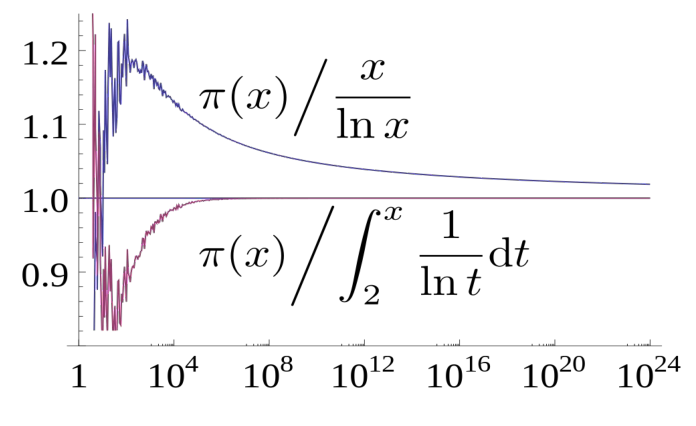
\includegraphics[width=0.40\textwidth]{pnt1.png}
		 \caption{$\pi(x)$ 与两个近似值的比例的图像}
\end{figure}

\subsection{发展历程}
1797年至1798年间, 法国数学家勒让德根据素数表猜测 $\pi (x)$ 具有 $\frac{x}{A\ln x + B}$ 的形式 (其中 $A,B$ 是参数).高斯也自称在15岁或16岁(1792或1793年)的时候考虑过类似的问题.1832年, 狄利克雷经过跟高斯的交流之后, 给出了一个新的逼近函数 $Li(x)$ (事实上他是用一个有点不一样的级数表达式)
\par 1859年, 黎曼提交了一篇关于素数分布的非常重要的报告《论小于给定数值的素数个数》, 这也是黎曼在这个领域的唯一一篇文章, 但这篇文章有着举足轻重的地位.黎曼在报告中使用了创新的想法, 将
 $\zeta$ 函数的定义解析延拓到整个复平面,并且将素数的分布与
 $\zeta$ 函数的零点紧密的联系起来, 具体来说是 $\zeta $ 函数在 $z = 1 + \i t (t>0)$ 这些复数上的取值都非零.这篇报告是历史上首次用复分析的方法研究实函数 $\pi(x)$, 对后来数论的研究影响深远.
\end{document}
